% use "latex" to generate a *.dvi file, and use "dvisvgm --no-fonts" to convert to .svg
\documentclass[border=10pt]{standalone}
\usepackage{tikz}

\begin{document}

\centering

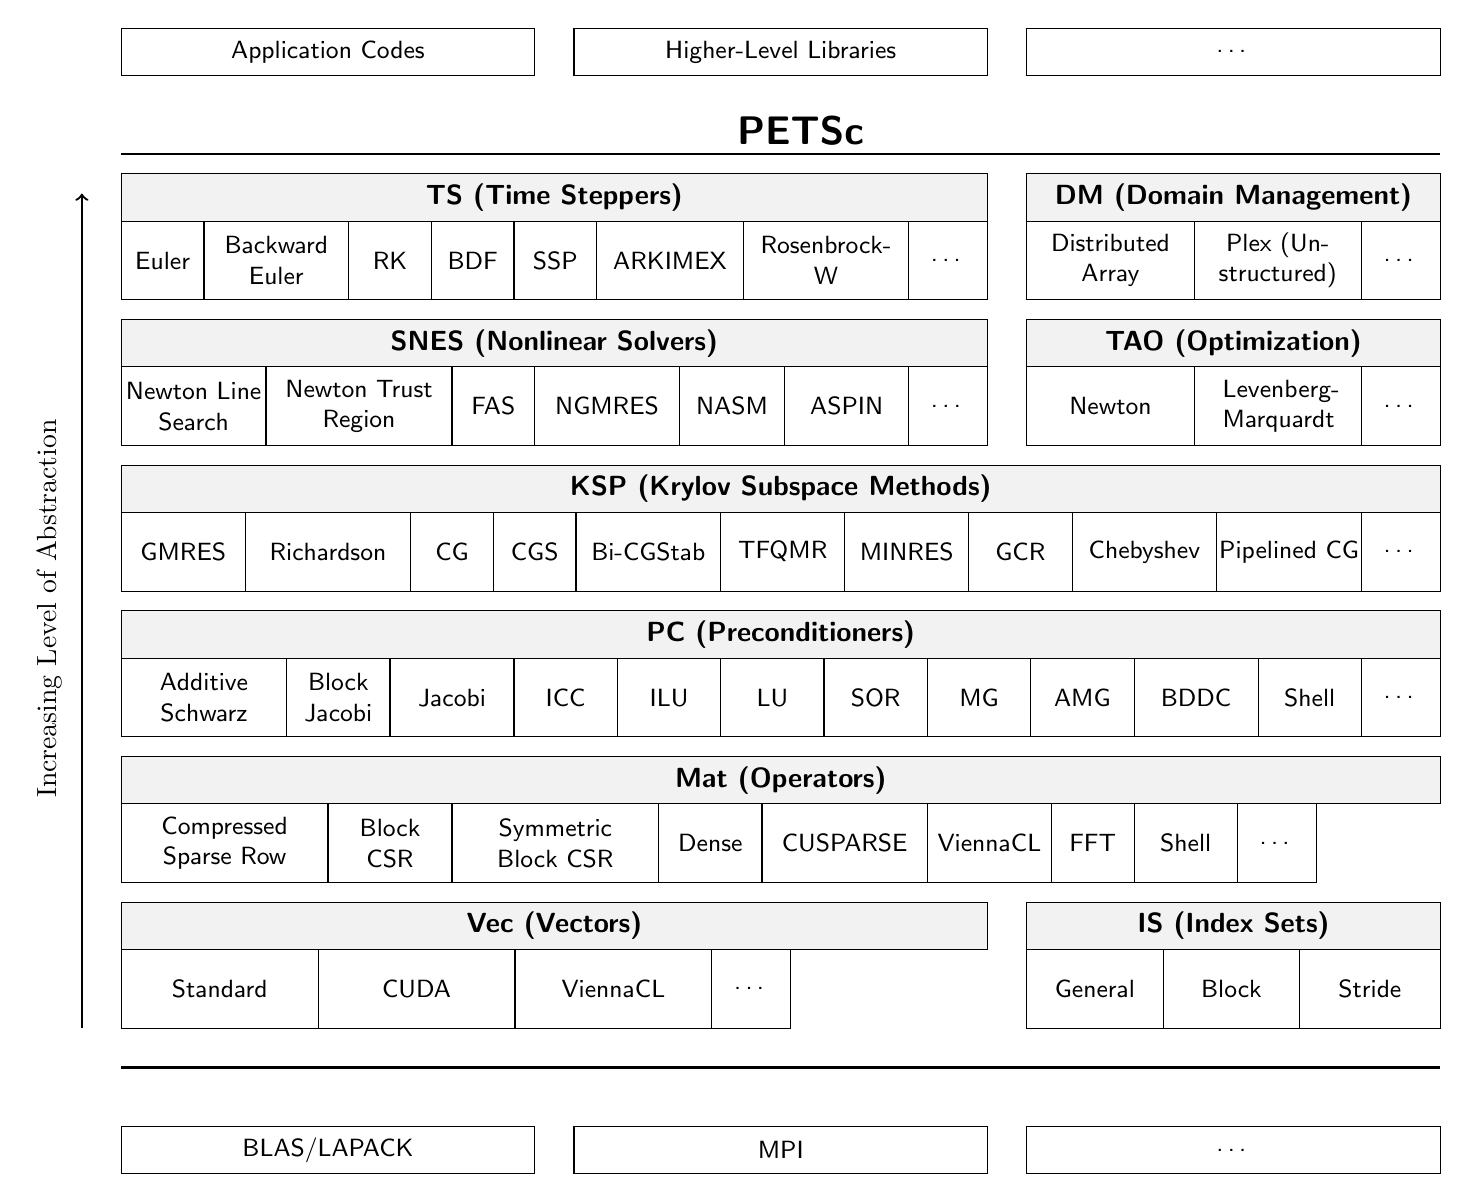
\begin{tikzpicture}
  \tikzstyle{interface}=[fill=black!5,font=\sffamily\bfseries]
  \tikzstyle{implem}=[font=\sffamily\small,text badly centered]
  \tikzstyle{ext}=[font=\sffamily\small]
  \tikzstyle{every node}=[transform shape]
  \def\levsep{1.85} % separation of levels
  \def\spacer{0.5}
  \def\block{5.25}
  \def\hint{0.6} % height interface
  \def\himp{1} % height implementation
  \draw[thick,->](-\spacer,0) -- (-\spacer,6*\levsep-\spacer) node[rotate=90,anchor=north,xshift=-150,yshift=20] {Increasing Level of Abstraction};
  \draw[ext] (0                 ,-\levsep) rectangle node {BLAS/LAPACK} +(\block,\hint);
  \draw[ext] (\block+\spacer    ,-\levsep) rectangle node {MPI}         +(\block,\hint);
  \draw[ext] (2*\block+2*\spacer,-\levsep) rectangle node {\dots}         +(\block,\hint);
  \draw[thick] (0,-\spacer) -- (3*\block+2*\spacer,-\spacer);
  \draw[interface] (0,\himp) rectangle node {Vec (Vectors)} +(2*\block+\spacer,\hint);
  \draw[implem] (0,0) rectangle node {Standard} ++(0.5*\block-0.25*\spacer,1) ++(0,-1)
                      rectangle node {CUDA} ++(0.5*\block-0.25*\spacer,1) ++(0,-1)
                      rectangle node {ViennaCL} ++(0.5*\block-0.25*\spacer,1) ++(0,-1)
                      rectangle node {\dots} ++(2*\spacer,1);
  \draw[interface] (2*\block+2*\spacer,\himp) rectangle node {IS (Index Sets)} +(\block,\hint);
  \draw[implem] (2*\block+2*\spacer,0) rectangle node {General} ++(0.33*\block,1) ++(0,-1) 
                rectangle node {Block} ++(0.33*\block,1) ++(0,-1)
                rectangle node {Stride} ++(0.34*\block,1);
  \draw[interface] (0,\levsep+\himp) rectangle node {Mat (Operators)} +(3*\block+2*\spacer,\hint);
  \draw[implem] (0,\levsep) rectangle node[text width=2.5cm] {Compressed Sparse Row} ++(0.5*\block,1) ++(0,-1) 
                rectangle node[text width=1.3cm] {Block CSR} ++(0.3*\block,1) ++(0,-1) 
                rectangle node[text width=2.3cm] {Symmetric Block CSR} ++(0.5*\block,1) ++(0,-1) 
                rectangle node {Dense} ++(0.25*\block,1) ++(0,-1) 
                rectangle node {CUSPARSE} ++(0.4*\block,1) ++(0,-1) 
                rectangle node {ViennaCL} ++(0.3*\block,1) ++(0,-1) 
                rectangle node {FFT} ++(0.2*\block,1) ++(0,-1) 
                rectangle node {Shell} ++(0.25*\block,1) ++(0,-1) 
                rectangle node {\dots} ++(2*\spacer,1) ++(0,-1);
  \draw[interface] (0,2*\levsep+\himp) rectangle node {PC (Preconditioners)} +(3*\block+2*\spacer,\hint);
  \draw[implem] (0,2*\levsep) rectangle node[text width=1.7cm] {Additive Schwarz} ++(0.4*\block,1) ++(0,-1) 
                rectangle node[text width=1.7cm] {Block Jacobi} ++(0.25*\block,1) ++(0,-1) 
                rectangle node {Jacobi} ++(0.3*\block,1) ++(0,-1) 
                rectangle node {ICC} ++(0.25*\block,1) ++(0,-1) 
                rectangle node {ILU} ++(0.25*\block,1) ++(0,-1) 
                rectangle node {LU} ++(0.25*\block,1) ++(0,-1) 
                rectangle node {SOR} ++(0.25*\block,1) ++(0,-1) 
                rectangle node {MG} ++(0.25*\block,1) ++(0,-1) 
                rectangle node {AMG} ++(0.25*\block,1) ++(0,-1) 
                rectangle node {BDDC} ++(0.3*\block,1) ++(0,-1) 
                rectangle node {Shell} ++(0.25*\block,1) ++(0,-1) 
                rectangle node {\dots} ++(2*\spacer,1);
  \draw[interface] (0,3*\levsep+\himp) rectangle node {KSP (Krylov Subspace Methods)} +(3*\block+2*\spacer,\hint);
  \draw[implem] (0,3*\levsep) rectangle node {GMRES} ++(0.3*\block,1) ++(0,-1) 
                rectangle node {Richardson} ++(0.4*\block,1) ++(0,-1) 
                rectangle node {CG} ++(0.2*\block,1) ++(0,-1) 
                rectangle node {CGS} ++(0.2*\block,1) ++(0,-1) 
                rectangle node {Bi-CGStab} ++((0.35*\block,1) ++(0,-1) 
                rectangle node {TFQMR} ++(0.3*\block,1) ++(0,-1) 
                rectangle node {MINRES} ++(0.3*\block,1) ++(0,-1) 
                rectangle node {GCR} ++(0.25*\block,1) ++(0,-1) 
                rectangle node {Chebyshev} ++(0.35*\block,1) ++(0,-1) 
                rectangle node[text width=1.8cm] {Pipelined CG} ++(0.35*\block,1) ++(0,-1) 
                rectangle node {\dots} ++(2*\spacer,1);
  \draw[interface] (0,4*\levsep+\himp) rectangle node {SNES (Nonlinear Solvers)} +(2*\block+\spacer,\hint);
  \draw[implem] (0,4*\levsep) rectangle node[text width=1.8cm] {Newton Line Search} ++(0.35*\block,1) ++(0,-1) 
                rectangle node[text width=2cm] {Newton Trust Region} ++(0.45*\block,1) ++(0,-1) 
                rectangle node {FAS} ++(0.2*\block,1) ++(0,-1) 
                rectangle node {NGMRES} ++(0.35*\block,1) ++(0,-1) 
                rectangle node {NASM} ++(0.35*\block-\spacer,1) ++(0,-1) 
                rectangle node {ASPIN} ++(0.3*\block,1) ++(0,-1) 
                rectangle node {\dots} ++(2*\spacer,1);
  \draw[interface] (2*\block+2*\spacer,4*\levsep+\himp) rectangle node {TAO (Optimization)} +(\block,\hint);
  \draw[implem] (2*\block+2*\spacer,4*\levsep) rectangle node[text width=1.2cm] {Newton} ++(0.5*\block-\spacer,1) ++(0,-1) 
                rectangle node[text width=1.4cm] {Levenberg-Marquardt} ++(0.5*\block-\spacer,1) ++(0,-1)
                rectangle node {\dots} ++(2*\spacer,1);
  \draw[interface] (0,5*\levsep+\himp) rectangle node {TS (Time Steppers)} +(2*\block+\spacer,\hint);
  \draw[implem] (0,5*\levsep) rectangle node {Euler} ++(0.2*\block,1) ++(0,-1) 
                rectangle node[text width=1.5cm] {Backward Euler} ++(0.35*\block,1) ++(0,-1) 
                rectangle node[text width=1.8cm] {RK} ++(0.2*\block,1) ++(0,-1) 
                rectangle node[text width=1.8cm] {BDF} ++(0.2*\block,1) ++(0,-1) 
                rectangle node[text width=1.8cm] {SSP} ++(0.2*\block,1) ++(0,-1) 
                rectangle node[text width=1.8cm] {ARKIMEX} ++(0.45*\block-\spacer,1) ++(0,-1) 
                rectangle node[text width=1.8cm] {Rosenbrock-W} ++(0.4*\block,1) ++(0,-1) 
                rectangle node {\dots} ++(2*\spacer,1);
  \draw[interface] (2*\block+2*\spacer,5*\levsep+\himp) rectangle node {DM (Domain Management)} +(\block,\hint);
  \draw[implem] (2*\block+2*\spacer,5*\levsep) rectangle node[text width=1.7cm] {Distributed Array} ++(0.5*\block-\spacer,1) ++(0,-1) 
                rectangle node[text width=1.7cm] {Plex (Unstructured)} ++(0.5*\block-\spacer,1) ++(0,-1)
                rectangle node {\dots} ++(2*\spacer,1);
  \draw[thick] (0,6*\levsep) -- (3*\block+2*\spacer,6*\levsep);
  \node[above,text centered,font=\sffamily\bfseries\Large] at (1.5*\block+1.5*\spacer,6*\levsep) {PETSc};
  \draw[ext] (0,6*\levsep+2*\spacer) rectangle node {Application Codes} +(\block,\hint);
  \draw[ext] (\block+\spacer,6*\levsep+2*\spacer) rectangle node {Higher-Level Libraries} +(\block,\hint);
  \draw[ext] (2*\block+2*\spacer,6*\levsep+2*\spacer) rectangle node {\dots} +(\block,\hint);
\end{tikzpicture}

\end{document}
